\documentclass[10pt, b5paper, openany]{ltjsbook}

\usepackage[T1]{fontenc}
\usepackage[utf8]{inputenc}
\usepackage[backend=biber, maxnames=100, backref=true]{biblatex}
\usepackage[binary-units = true]{siunitx}
\usepackage{amsmath, amssymb, amsthm}
\usepackage{graphicx}
\usepackage{hyperref}
\usepackage{ascmac}
\usepackage{here}
\usepackage{comment}

\setlength{\textwidth}{\fullwidth}
\setlength{\evensidemargin}{\oddsidemargin}

\DeclareGraphicsRule{.ai}{pdf}{.ai}{}

\title{ \LaTeX Sample1 } 
\author{ komekome09(こめわっぽ) }
\date{ \today }

\begin{document} %document環境
\chapter*{はじめに}
みなさんは美少女ゲームをやっていますか?(筆者は積みゲーばかりでほとんどやってません)
周囲の美少女ゲーマーは皆Windowsにゲームをインストールしてプレイしている人がほとんどです。
ですがゲームをプレイするためにWindows機を用意するのはかったるい!なんということだ!と感じた方も少なくは無いはずです(?)
そんな悩みを解決すべく、UEFIを採用したBIOS上のアプリで美少女ゲームを動かせるプラットフォームを作っていくぞ!
....という意気込みで始めました\footnote{執筆時点では完成とかそういうレベルではないです。}。

というわけでこの本ではUEFI Applicationを用いて美少女ゲーム(以降ノベルゲームと書きます)の土台のようなものを作ろうとしている記録を本にしたものです。
一応技術的な本ではありますが、内容が無いよう状態の本なのでそこの所は暖かい目で見守りつつ石を投げつけてくれると幸いです。

\tableofcontents
\clearpage

\chapter{結局どういうの作ったの}
\begin{figure}[H]
    \centering
    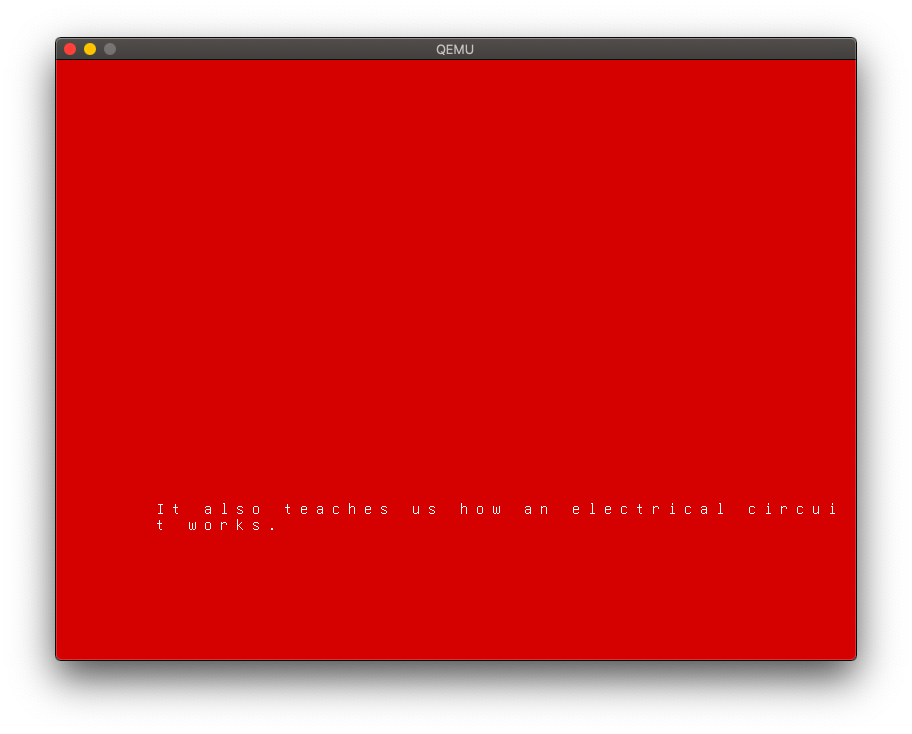
\includegraphics[scale=0.3]{pic/screenshot.png}
    \section{作成中の画面}
    \label{fig:screenshot}
\end{figure}
現状では画像の表示はできる、テキストもフォントに目を潰れば表示できている、音楽は全くの未対応という状況です。


\chapter{(最終的な)実装内容}
UEFI Application上でノベルゲームの土台を作るという目標ですが、具体的にどのような機能を実装すればいいのでしょうか。
まずそこから分からない状態だったので洗い出すことにしました。

ノベルゲームを構成する要素は大きく以下の3つが重要となるでしょう。
\begin{itemize}
    \item 画像
    \item BGM
    \item テキスト
\end{itemize}
まずはこれを足掛りとして考えていきます。

\section{前提}
UEFI Applicationを作る上の前提として、ほとんどのライブラリが使えないというのがあります。
実際にはEDK2のlibc移植だったり、自力でlibcを移植すればできなくもないですがどつぼにはまると大変なことになります(筆者はなりました)。
ですので今回は「この程度だったら手作業での移植でもどうにかなるだろう…」という程度のライブラリ(など)を扱うようにしています。

\section{画像}
ノベルゲームだけに当てはまる話ではありませんが、ただ単に画像を表示して終わりで済むような場面はそこまで多くありません。
例えば以下の場面を考えてみましょう。
\begin{figure}[H]
    \centering
    \includegraphics[scale=0.3]{pic/nobel_exp.ai}
    \caption{ノベルゲームの表示例}
    \label{fig:nobel_exp}
\end{figure}
基本的にノベルゲームではピンク色で塗られた画像が表示される部分と、橙色で上に塗られた文字などを表示する部分に分かれています。
また文字が表示される部分は背景の画像が見えるように透過されている場合もあります。

このように、ただ画像を表示するだけでなく透過処理などの処理が必要となる場合がほとんどです。

UEFI App上で作成する上では透過などの機能は基本的には自分で実装することになります(他の機能に関してもそうです)。
\section{BGM}
BGM
\section{テキスト}
テキスト処理、フォントなども用意する必要があります。
今回はBitmapFontが簡単にできるのでそれで文字を出せるようにしていますが、まあ見た目は…という感じになります。
本当ならTrueTypeフォントみたいなの使えればいいんですけどね(先駆者はいたはず)。

\section{結局何を実装するの}
\begin{itemize}
    \item 画像表示(jpg, png, bmp, 等々)
    \item BGM(wav, mp3, 等々)
    \item フォント処理
\end{itemize}
が実装すべき内容となります(最低限)。

\chapter{環境構築}
では実際にUEFI Applicationを作るための開発環境を構築していきます。
ライブラリはgnu-efi 3.0.7を使用します。
また実行ファイルはPE32+形式なため、Windows環境以外ではクロスコンパイラが必要となります。
今回はDocker上に開発環境を作成しました。

\chapter{コード}
\chapter{あとがき}

\begin{comment}
\section{見出し1}
    本文はこんな感じで入力します。\par
    改行をしたいときは、字下げを行う場合は \verb+\par+ 、そうでない場合は\verb+\\+ を使います。
    \subsection{小見出し1}
        見出しの中をさらに小分けができます。こういった分け方を「章立て」と呼び、日本語では大きい単位から「章」「節」「項」と言います。\par
        \LaTeX ではデフォルトでは1.1.2、といった形で表示され、この場合は第1章第1節第1項、と呼びます。
        \subsubsection{小々見出し1}
        \LaTeX{} is a document preparation system for the \TeX{} typesetting program. It offers programmable desktop publishing features and extensive facilities for automating most aspects of typesetting and desktop publishing, including numbering and cross-referencing, tables and figures, page layout, bibliographies, and much more. \LaTeX{} was originally written in 1984 by Leslie Lamport and has become the dominant method for using \TeX; few people write in plain \TeX{} anymore. The current version is \LaTeXe.
\section{基本的な文法}
    \subsection{箇条書き}
        箇条書きにはいくつか種類があります。
        \subsubsection{itemize}
            これは「・」が頭についた箇条書きです。
            \begin{itemize}
                \item 箇条書き1
                \item 箇条書き2
                \item 箇条書き3
            \end{itemize}
        \subsubsection{enumerate}
            これは頭に数字が振られている箇条書きのコマンドです。
            \begin{enumerate}
                \item 箇条書き1
                \item 箇条書き2
                \item 箇条書き3
            \end{enumerate}
        \subsubsection{description}
            これは頭につける記号をユーザが決めることができるコマンドです。
            \begin{description}
                \item[テスト1] 箇条書き1
                \item[テスト2] 箇条書き2
                \item[テスト3] 箇条書き3
            \end{description}
    \subsection{表組み}
        \subsubsection{基本的な表}
            \begin{table}[H]
                \begin{center}
                \caption{基本的な表}
                \begin{tabular}{|l|c|r|}
                    \hline
                    セル1 & セル2 & セル3 \\ \hline
                    セル4 & セル5 & セル6 \\ \hline
                    セル7 & セル8 & セル9 \\ \hline
                \end{tabular} 
                \end{center}
            \end{table}
        \subsubsection{セルの結合}
            \begin{table}[H]
                \begin{center}
                \caption{セルの結合}
                \label{tab:sample1}
                \begin{tabular}{|l|c|r|}
                    \hline
                     & \multicolumn{2}{|c|}{セル1} \\ \cline{2-3}
                    セル2 & セル3 & セル4  \\ \cline{2-2}
                     & セル5 &  \\ \hline
                \end{tabular} 
                \end{center}
            \end{table}
            表を参照するときはこうします(表\ref{tab:sample1})
        \subsubsection{複数の表}
        \begin{table}[H]
            \begin{center}
            \begin{tabular}{cc}
            
            \begin{minipage}{0.5\hsize}
            \begin{center}
            \begin{tabular}{|c|c|c|}
            \hline
            a & b & c \\ \hline
            d & e & f \\ \hline
            g & h & i \\ \hline
            \end{tabular}
            \caption{aが9つ}
            \end{center}
            \end{minipage}
            
            \begin{minipage}{0.5\hsize}
            \begin{center}
            \begin{tabular}{|c|c|c|}
            \hline
            j & k & l \\ \hline
            m & n & o \\ \hline
            p & q & r \\ \hline
            \end{tabular}
            \caption{bが9つ}
            \end{center}
            \end{minipage}
            
            \end{tabular}
            \end{center}
        \end{table}
    \subsection{数式}
        \subsubsection{その1}
            \begin{eqnarray}
                G_{-1}(x,y)=x^{n-1}+x^n-1
                \label{eq:sample1}
            \end{eqnarray}
                
            \begin{eqnarray}
                W(D)&=&(I(D),(1+D)I(D)) \nonumber \\
                &=&I(D)[1,1+D] \nonumber \\
                &=&I(D)G(D)
            \end{eqnarray} 
            
            \[
            x=a+b+c
            \]
            
            本文中にも数式を$ x=a+b+c $表示できます。\par
            数式の参照はこうやります(式(\ref{eq:sample1}))            
        \subsubsection{その2}
            \begin{eqnarray}
                y=\frac{\sqrt[2]{1+x}}{1-x}
                \end{eqnarray} 
                
                \begin{eqnarray}
                \left(\frac{1+x}{1-x}\right) +(\frac{1-x}{1+x})
                \end{eqnarray} 
                
                \begin{eqnarray}
                c_{k,l}=\left\{ \begin{array}{ll}
                1[\mathrm{m/s]}] & (l=k) \\
                \alpha & (|l-k|=1) \\
                0[\mathrm{m/s]} & (上記以外) \\
                \end{array} \right.
            \end{eqnarray}
    \subsection{画像の挿入}
        \begin{figure}[H]
            \begin{center}
            %\includegraphics[width=5cm]{figure1.jpg}
            \end{center}
            \caption{図の説明}
            \label{fig:sample1}
        \end{figure}
        画像の参照はこうやります(図\ref{fig:sample1})
\section{参考文献の参照}
    参考文献を参照する場合は\cite{bib1}こうします。
\section{その他のコマンド}
    その他特殊文字や細かい操作方法などは\cite{sheat1,sheat2}を参照してください。

\begin{thebibliography}{9}
    \bibitem{bib1} ここに参考文献を入力します
    \bibitem{sheat1} unknown, `` LaTeXコマンドシート一覧,'' 2003, [online] Available: \url{http://www002.upp.so-net.ne.jp/latex/index.html}
    \bibitem{sheat2} unknown, `` LaTeXコマンド集,'' 2009, [online] Available: \url{http://www.latex-cmd.com}
\end{thebibliography}
\end{comment}
\end{document}

